\documentclass[]{article}
%Font encoding for swedish
\usepackage[utf8]{inputenc}
\usepackage[swedish]{babel}
\usepackage[T1]{fontenc}

%For source code boxes
\usepackage{listings}

\usepackage{mdwlist}

\usepackage{multicol}
\usepackage{fancyvrb}
\usepackage{hyperref}

\usepackage{framed}

\usepackage{tikz}
\usetikzlibrary{shapes,arrows,calc}

\usepackage[titletoc,title]{appendix}


% Title Page
\title{Teknisk rapport\\Grafisk räknare}
\author{}


\begin{document}
\maketitle

\begin{abstract}
\end{abstract}
\section{Inledning}
Bakgrund, syfte, källor!?
\section{Apparaten}
\begin{figure}[h!]
	\makebox[\textwidth][c]{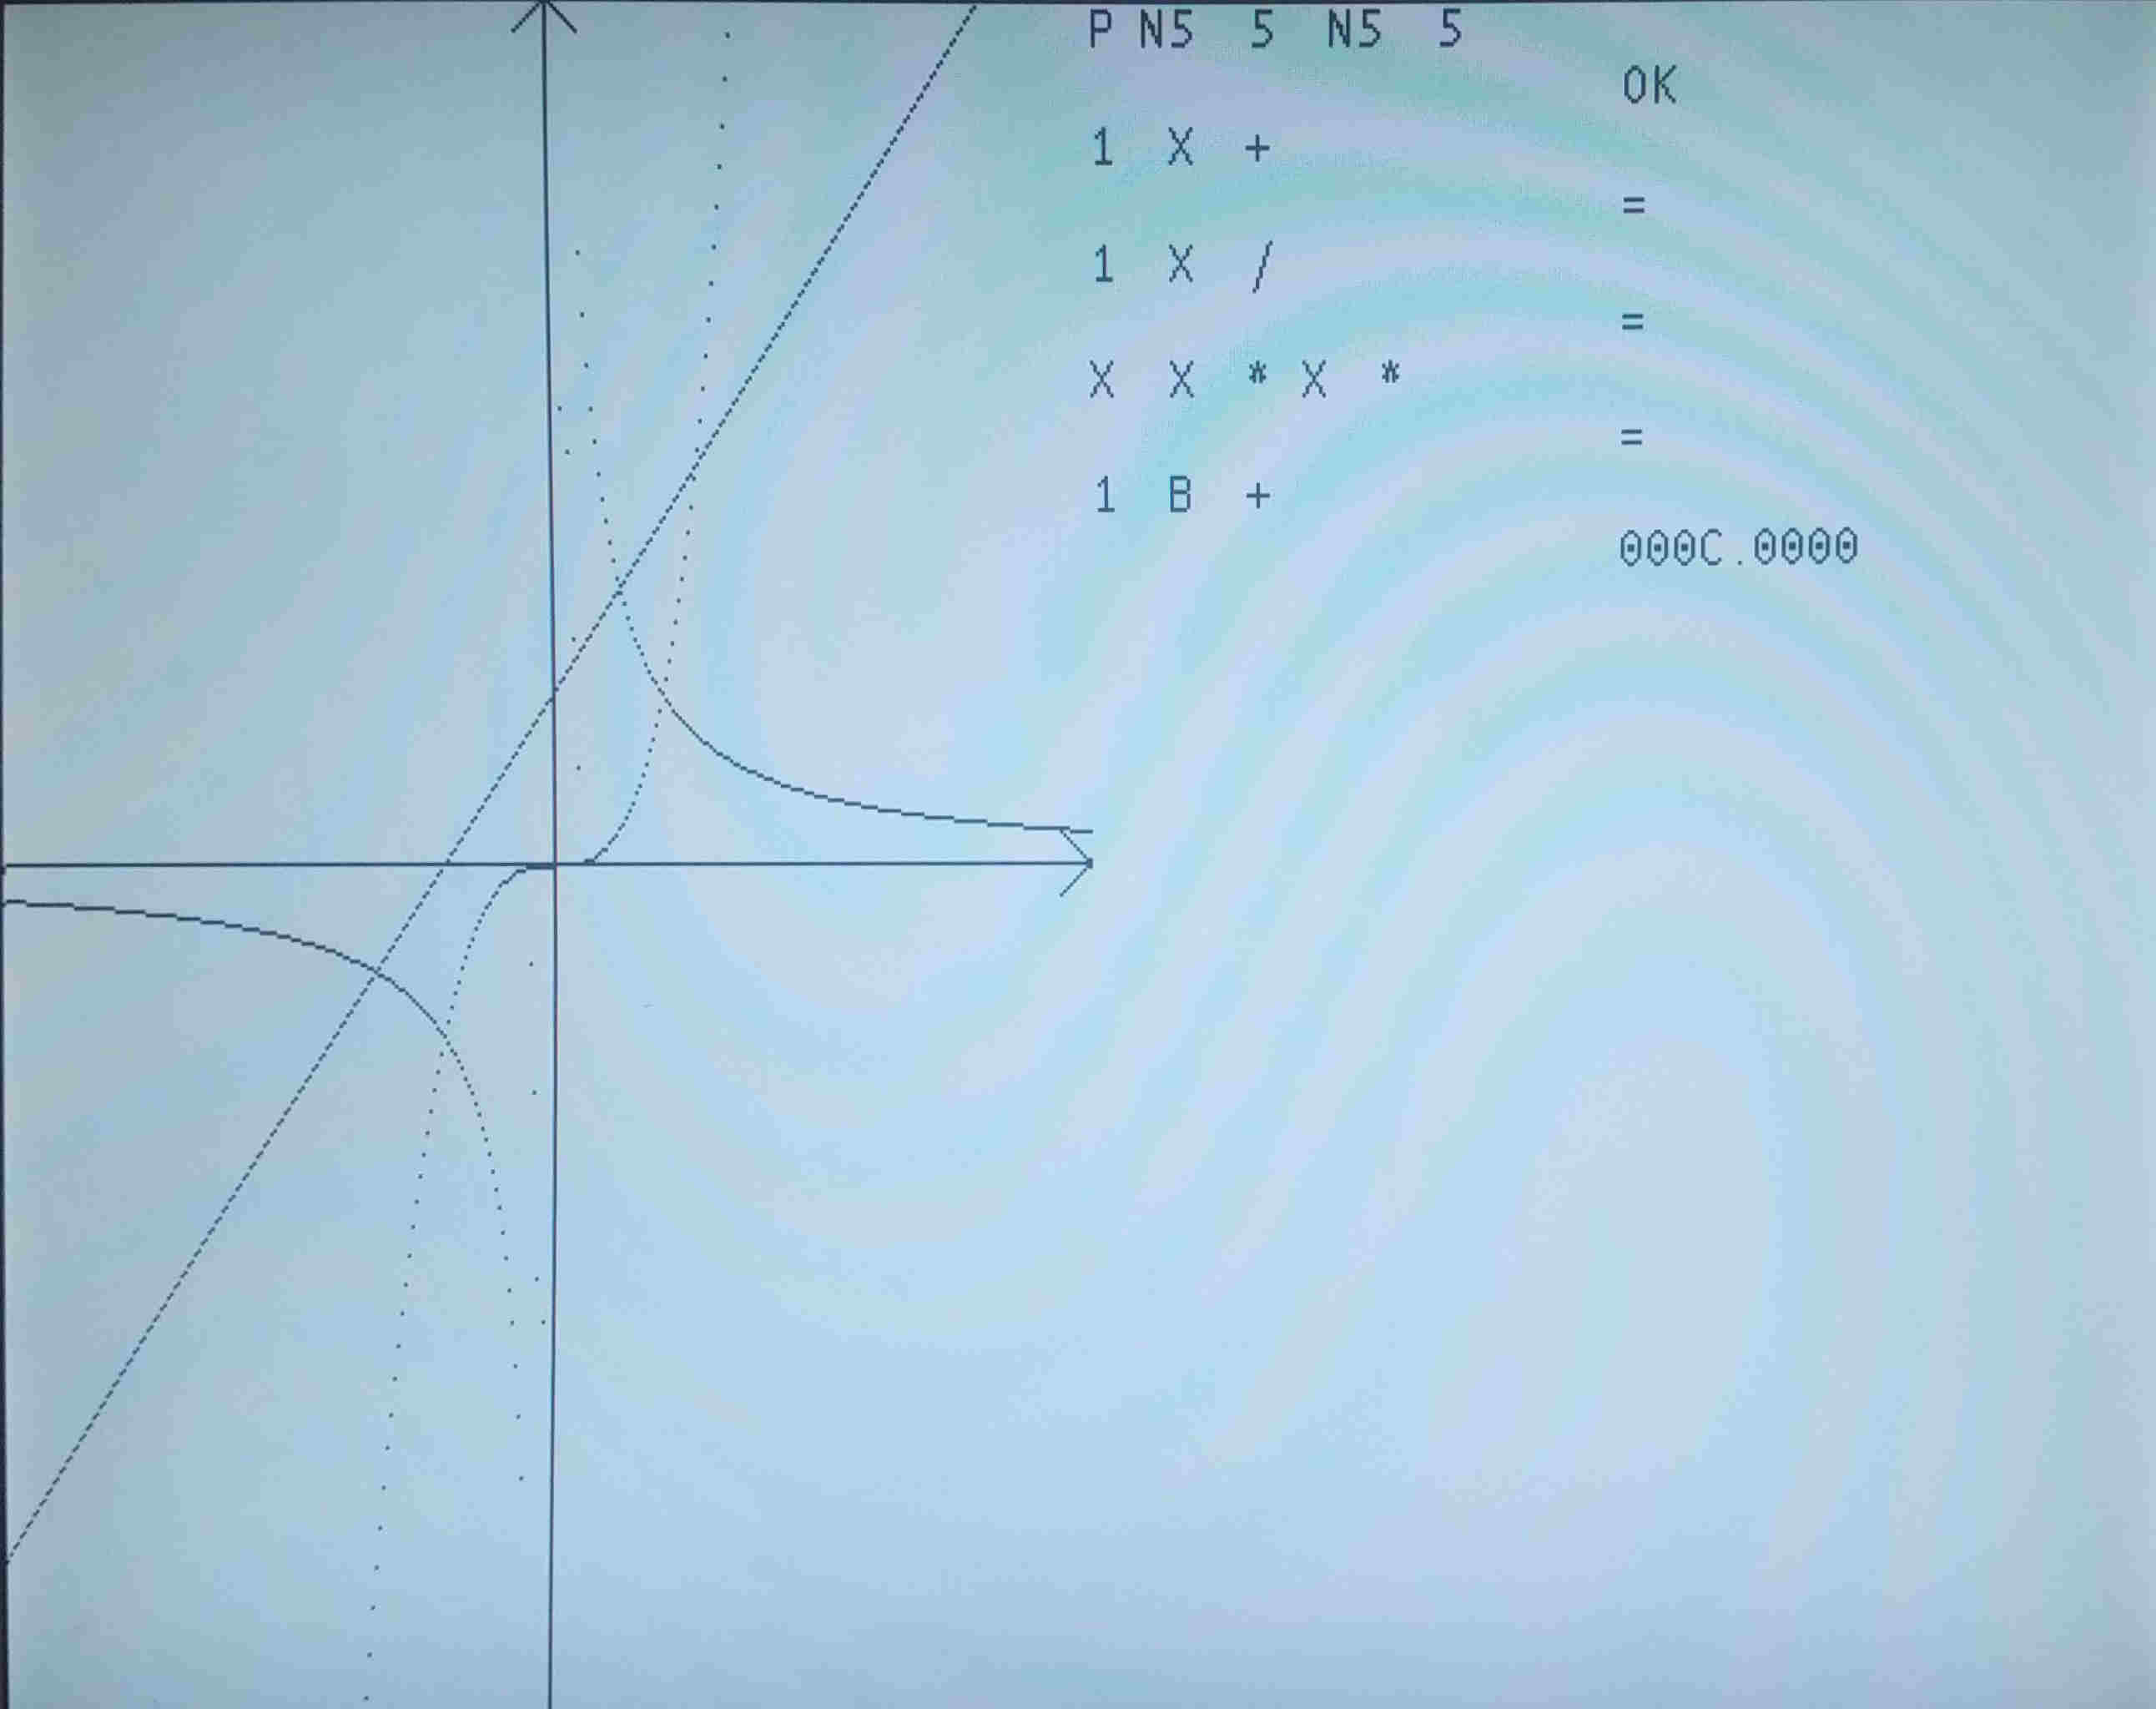
\includegraphics[width=0.8\textwidth]{drawings/display_lq.jpg}}
	\caption{Bild på grunkan \textbf{TODO: Low quality because sshfs is slow. Change to HQ when done}}
\end{figure}
Apparaten är en hexadecimal grafräknare med reverse polish-notation.

Börja gärna med en bild på bygget och redgör för hur apparaten används. Detta blir en kombinerad presentation av konstruktionen och användarhandledning. 

\subsection{Beräkningar och inmatning}
\begin{figure}[h!]
	\makebox[\textwidth][c]{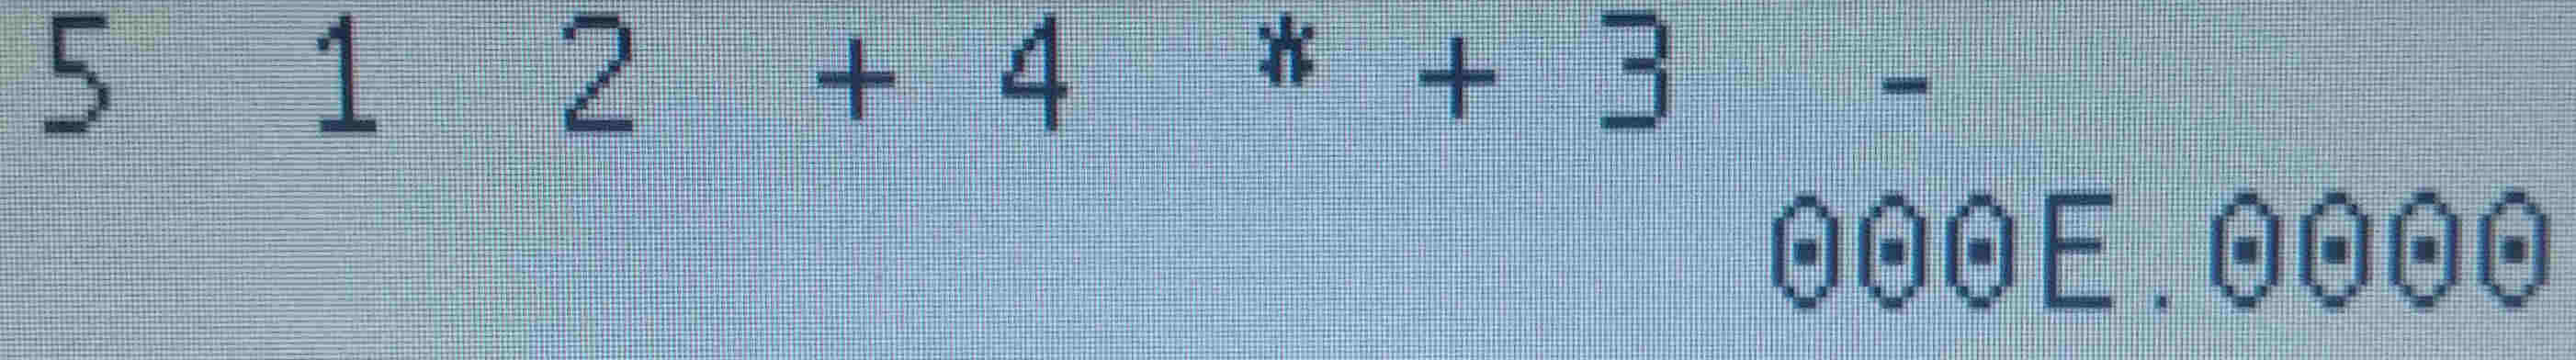
\includegraphics[width=0.8\textwidth]{drawings/calculation_lq.jpg}}
	\caption{Beräkningsexempel \textbf{TODO: Low quality because sshfs is slow. Change to HQ when done}}
\end{figure}
En vanlig beräkning genomför genom att man skriver ett uttryck och avslutar med enter. 

Siffror skrivs in med numpad eller sifferraden, tillsammans med knapparna \texttt{A-F}. För att få negativa tal börjar man med ett \texttt{N} innan siffrorna. Decimalen fås med punkt. Avsluta siffor med mellanslag. Notera att endast siffror upp till 32 bitars tvåkomplement stöds, med jämn uppdelning mellan heltalsdelen och decimaldelen. Med andra ord går heltalsdelen från $-8000$ och $+7FFF$, medan decimaldelen går mellan $0000$ och $FFFF$.

Operander matas in via knapparna på numpaden. Efter dessa behövs inget mellanslag.

\subsection{Grafritning}
En funktion för uppritning matas in likadant som en vanlig beräkning, med undantag för att en eller flera siffror ersätts med \texttt{X}. Som standard kommer den inmatade funktionen ritas mellan $-10$ och $10$ i både X- och Y-led.

Vill man ändra utritningsområdet så görs det genom att man matar in 
\begin{Verbatim}[frame=single]
P Xmin Xmax Ymin Ymax
\end{Verbatim}
där Xmin, Xmax, Ymin och Ymax skrivs in som vanliga siffror. P räknas som operator och ska alltså inte ha något mellanslag efter sig. När den fjärde siffran matats in så töms grafen och nästa funktion som matas in kommer att ritas på det nya utritningsområdet.

\section{Teori}
Här kan ett videoprojekt beskriva videoformatet, ett MIDI-projekt redogöra för MIDI-standarden ...
\subsection{Reverse polish}
Reverse polish är en notation för aritmetiska uttryck utan parenteser. Även känt som postfixnotation, eftersom operatorn hamnar efter operanderna. Exempelvis skrivs $1+2$ som $1 2 +$. Har man flera operatorer så skrivs operatorn direkt efter andra operanden, exempelvis $1-2+3$ blir $1 2 - 3 +$. Man läser alltså från vänster till höger. När det kommer en operand så appliceras den på de två värdena som kom innan, och resultatet läggs tillbaka på operandens plats. Ett mer avancerat exempel med parenteser är $5 + ((1 + 2) * 4) - 3$ som blir $5 1 2 + 4 * + 3 -$.\footnote{Källa: \href{https://en.wikipedia.org/wiki/Reverse_Polish_notation}{\url{https://en.wikipedia.org/wiki/Reverse_Polish_notation}}}
\section{Hårdvaran}
Börja med ett översiktligt blockschema, gå vidare till mera detaljerade blockschemor. Vill man rita figurer och blockschemor på datorn så är Inkscape ett bra alternativ. Handritade figurer och blockschemor är acceptabelt, bara de är snygga och väl läsbara, MEN dessa ska då vara inscannade, dvs avfotograferade figurer och blockschemor är INTE godtagbart.
Beskriv sedan hur de olika blocken fungerar. Tänk på läsbarheten och växla mellan figurer och text. Den här typen av text är ganska "grafisk", då nästan varje mening syftar in i en figur. Var därför noga med att text och figurer stämmer överens.
\subsection{Översikt}

\tikzstyle{block} = [draw, fill=blue!20, rectangle, 
minimum height=3em, minimum width=6em]
\tikzstyle{sum} = [draw, fill=blue!20, circle, node distance=1cm]
\tikzstyle{input} = [coordinate]
\tikzstyle{output} = [coordinate]
\tikzstyle{pinstyle} = [pin edge={to-,thin,black}]

\begin{figure}[h!]
	\centering
	\begin{tikzpicture}[auto, node distance=2cm,>=latex']
	
	
	
	\node [block, node distance=3cm] (cpu) {CPU};
	\node [block, below of=cpu, node distance=2cm] (memory) {Bildminne};
	\node [output, right of=cpu] (foo) {};
	
	
	\draw [<->] (cpu) -- node[near start]{} (memory);
	\node [block, above of=cpu] (keyboarddriver) {Tangentbordsmotor};
	\node [block, node distance=3.5cm, left of=keyboarddriver] (keyboard) {Tangentbord};
	
	\draw [<->] (keyboarddriver) -- node {} (cpu);
	\draw [->] (keyboard) -- node {} (keyboarddriver);
	
	\node [block, node distance=2cm, below of=memory] (driver) {VGA-motor};
	\node [block, right of=driver, node distance=3.5cm] (vga) {Skärm};
	\draw [<->] (memory) -- node {} (driver);
	\draw [->] (driver) -- node {} (vga);
	\draw[thick,dotted] ($(keyboarddriver.north west)+(-0.3,0.3)$)  rectangle ($(driver.south east)+(1,-0.3)$) node[pos=0] {FPGA};
	\end{tikzpicture}
	\caption{Översiktligt blockschema.}
\end{figure}

\subsection{CPU}

CPU:n är baserad på icke-pipelinade Björn Lindskogs-datorn. Huvudminnet, och de allra flesta register inklusive de generella, är 32 bitar långa.

\subsubsection{mPC}

Microprogramräknaren. Microninstruktioner har fyra bitar att modifiera räknaren med, vilket sker på positiv klockflank. Koderna gör som följer:
\\

\begin{tabular}{ll}
	\textbf{Kod}    & \textbf{Funktion}                              \\ \hline
	\texttt{0001}   & mPC := ADR                                     \\
	\texttt{0010}   & mPC := K2(<Given mod>)                         \\
	\texttt{0011}   & mPC := K1(<Given Instruktion>)                 \\
	\texttt{1000}   & mPC := ADR if flag\_X == \texttt{1} else mPC++ \\
	\texttt{1001}   & mPC := ADR if flag\_N == \texttt{1} else mPC++ \\
	\texttt{1010}   & mPC := ADR if flag\_Z == \texttt{1} else mPC++ \\
	\texttt{1011}   & mPC := ADR if flag\_C == \texttt{1} else mPC++ \\
	\texttt{1100}   & mPC := ADR if flag\_V == \texttt{1} else mPC++ \\
	\texttt{Others} & mPC++
\end{tabular}
\\

\noindent
K2 och K1 är minnen som binder en given mods eller instruktions binärrepresentation till raden i microminnet som har hand om dess del i hämtfasen respektive exekveringsfasen.

\subsubsection{IR}

Instruktionsregistret, 32 bitar, håller i en kopia av instruktionen från huvudminnet som körs för tillfället. Den kan vidare delas upp i OP, GRx och MM som är den instrukionens instruktionskod, GRx-argument samt valt mod.

Man kan i microkoden skriva och läsa till och från IR genom att ange busskoden \texttt{0001} i från-buss respektive till-bus fältet. Att skriva till IR påverkar inte huvudminnet, och därmed inte den egentliga programkoden.

\subsubsection{PC}

Programräknaren, håller koll på instruktion i p\_mem som ska exkaveras. Registret är 22 bitar långt, då detta är fullt tillräckligt för alla rimligt stora program, samt att addressfältet hos en instruktion inte har plats för större tal på sin addressdel: de sista 22 bitarna.

PCsig, bit nummer 18 i microinstruktionen, kan påverka PC. Ett värde på 0 håller PC oförändrad, medan ett värde på 1 inkrementerar den.

PC kan skrivas till via bussen. En från-buss-signal på \texttt{0011} skriver de 22 lägsta bitarna av DATA\_BUS till PC. Den kan även läsas ifrån genom att ange samma busskod på till-buss delen i microminnet.

\subsubsection{ASR}

Addressregistret används i microprocessorn för att peka ut addressen till raden som ska passera som argument. Detta sätts i hämtfasen och beror på vilket mod den dåvarande instruktionen körs med.

Liksom PC är registret av samma anledning 22 bitar långt.

ASR kan läses från och skrivas till via busskoden \texttt{0100}.

\subsubsection{GRx}

De åtta generella registrena: GR0 till och med GR7.

Dessa register är 32 bitar långa och används för att främst hålla i temporära värden åt användaren.

Vektorn g\_reg håller i de åtta registren, och ett av de väljs genom signalen GRx. Denna är bitar 26 till och med 24 hos programinstruktionen som körs för tillfället.

Att skriva eller läsa till det valda generella registret görs via busskuden \texttt{1000}. Det är den som valts i GRx som då interageras med. 

\subsubsection{p\_mem}

Vårt programminne, 32 bitar långt. Då programminne och dataminne är samma minne så syftas här på det delade minnet. Genom att skriva eller läsa härifrån via busskoden \texttt{0010} så kan huvudminnet läsas eller modifieras. Raden i minnet som opereras på utpekas ASR, som sätts automatiskt i hämtfasen.

Det är värt att notera att programminnet initialt sätts till konstanten p\_mem\_c, där då programkod skrivs in.

\subsubsection{save\_at\_p/save\_at\_b/data\_out\_picmem/data\_out\_bitmap}

Signaler för att skriva till bild och bitmapminne. Via busskoden \texttt{0111} skickas de sista 8 bitarna i \texttt{DATA\_BUS} via \texttt{data\_out\_picmem} och \texttt{ASR} till \texttt{save\_at\_p}. Via busskoden \texttt{0110} skickas den sista biten i \texttt{DATA\_BUS} via \texttt{data\_out\_bitmap} och \texttt{ASR} till \texttt{save\_at\_b}. Samtidigt aktiveras en (aktivt hög) write-enable-signal, \texttt{web} vid skrivning till bitmapminnet och \texttt{wep} vid skrivning till bildminnet. Dessa nollställs inte, utan används bara för att undvika odefinierade signaler innan första skrivningen.

\subsubsection{AR/ALU}

I processen titulerad AR finns koden som utgör enhetens ALU.

Här modifieras ackumulatorregistret, AR, (32 bitar), och de fem flaggorna. En rad olika operationer kan utföras på positiv klockflank beroende på koden hos ALU-signalen; de fem första bitarna i mikrominnesinstruktionen som för tillfället körs.

Vid matematiska operationer tolkas AR och bussens värde som ett signerat tvåkomplementstal.

AR:s värde kan senare läggas på bussen genom att ange koden \texttt{0101} i mikrokoden. Den kan dock ej skrivas till direkt.

Nedan följer en tabell över alla ALU-operationer: deras koder, funktion, och modifierade flaggor.
\\

\begin{tabular}{llc}
	\textbf{Kod}    & \textbf{Funktion}                                      & \textbf{Flaggor påverkade} \\ \hline
	\texttt{00000}  & \texttt{<Ingenting>}                                   &  \\
	\texttt{00001}  & AR := BUS                                              &  \\
	\texttt{00010}  & AR := BUS'                                             &  \\
	\texttt{00011}  & AR := 0                                                &  \\
	\texttt{00100}  & AR := AR+BUS                                           &     \texttt{X C V N Z}     \\
	\texttt{00101}  & AR := AR-BUS                                           &     \texttt{X C V N Z}     \\
	\texttt{00110}  & AR := AR \textsc{and} BUS                              &    \texttt{{ } C V N Z}    \\
	\texttt{00111}  & AR := \textit{signed\_to\_real}(AR) (16 skift vänster) &  \\
	\texttt{01000}  & AR := \textit{real\_to\_signed}(AR) (16 skift höger)   &  \\
	\texttt{01001}  & AR := AR \textsc{asr} BUS                              &     \texttt{X C V N Z}     \\
	\texttt{01010}  & AR := AR \textsc{asl} BUS                              &     \texttt{X C V N Z}     \\
	\texttt{01011}  & AR := AR+BUS (Ekvivalent med \texttt{00100})           &     \texttt{X C V N Z}     \\
	\texttt{01100}  & AR := AR-BUS (Ekvivalent med \texttt{00101})           &     \texttt{X C V N Z}     \\
	\texttt{01101}  & AR := AR*BUS (fixed point)                             &  \\
	\texttt{01110}  & \texttt{<Undefined>}                                   &  \\
	\texttt{01111}  & AR := AR \textsc{lsr} BUS                              &    \texttt{X C { } N Z}    \\
	\texttt{10000}  & AR := AR \textsc{lsl} BUS                              &    \texttt{X C { } N Z}    \\
	\texttt{Others} & \texttt{<Undefined>}                                   &
\end{tabular}
\\

TODO: Hälfen av det här gör ju identiska saker eller används aldrig (antingen i assembly eller inte ens i mikrokod)


\subsection{Tangentbordsmotor}
Tangentbordsmotorn i \texttt{KBD\_ENC} sköter inmatning från ett tangentbord över PS/2-protokollet. När en tangent trycks ner skickas 11 bitar seriellt över dataingången i tangentbordsmotorn, och klockingången klockas i takt med dessa så att databitarna kan läsas vid negativ flank på klockan. Av de 11 bitarna är den första biten en startbit som alltid är 0. Efter startbiten följer 8 databitar (mest signifikant bit skickas först)  som utgör den aktuella scankoden\footnote{\url{http://www.computer-engineering.org/ps2keyboard/scancodes2.html}}, och till sist en paritetsbit (udda paritet) och en stoppbit som alltid är 1.

När alla 11 bitar har lästs av tangentbordsmotorn går scankoden vidare till en tillståndsmaskin som avgör om \texttt{MAKE} eller \texttt{BREAK} (dvs. om den aktuella tangenten trycks ner eller släpps). Denna process kan endast avgöra tillståndet för en tangent åt gången, och flera knapptryckningar samtidigt stödjs således inte. Scankoden översätts sedan till motsvarande tile i bildminnet.

Om tidigare nämnda tillståndsmaskin bestämde att \texttt{MAKE} har inträffat läggs tilekoden på tangentbordsmotorns datautgång och hålls där för att vid senare tillfälle läsas av CPU:n. Tilekoden hålls på bussen tills tangentbordsmotorn antingen får en återställningssignal från Nexyskortet eller processorn skickar en 1:a över \texttt{read\_confirm}-signalen (denna signal skickas automatiskt av \texttt{RC}-instruktionen). Efter en sådan återställning sätts bussen till värdet x$FF$ som hålls tills en ny tangent registreras. Detta tillvägagångssätt medför att processorn alltid kan läsa av den senaste nedtryckta tangenten med \texttt{RC}.

\begin{figure}[h!]
	\makebox[\textwidth][c]{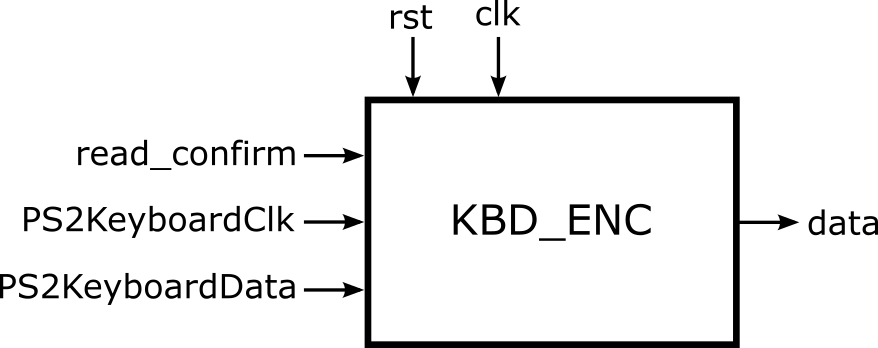
\includegraphics[scale=1]{drawings/kbd_enc.png}}
	\caption{Övergripande blockschema över tangentbordsmotorn}
\end{figure}

\subsection{Bildminne}
\begin{figure}[h!]
	\makebox[\textwidth][c]{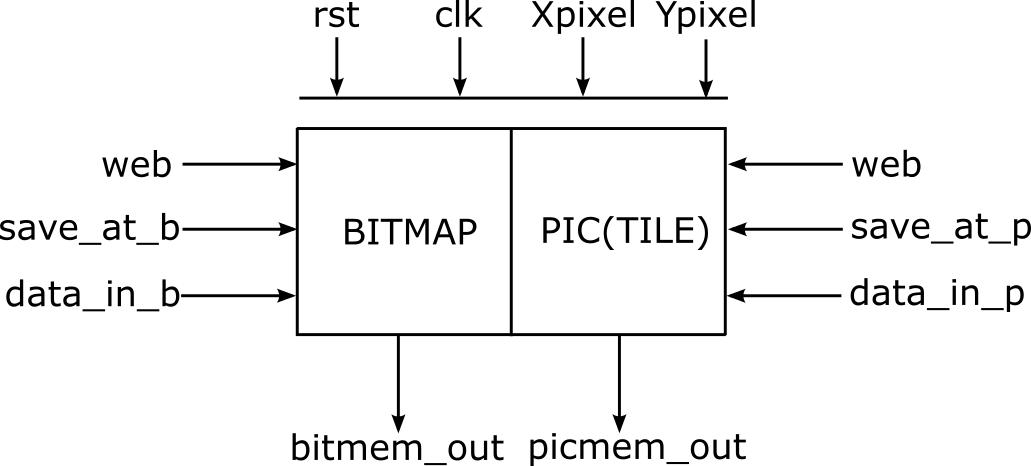
\includegraphics[width=1\textwidth]{drawings/pic_mem.png}}
	\caption{Blockschema över bildminnet}
\end{figure}

Bildminnet är uppdelat i två kolumner, där ena hälften använder tiles och andra hälften använder en bitmap. Bitmapminnet innehåller 320x480 bitars blockram för en svartvit representation av alla pixlar på vänstra skärmhalvan. Bildminnet för tiles innehåller 40x30 rader.

Varje del har en write\_enable-signal, en save\_at-signal och en data\_in-signal. När write\_enable ettställs ersätts innehållet på adressen save\_at med data\_in. Ingen kontroll av att adresserna ligger inom minnet sker, utan det är upp till programmeraren.

\label{parag:picmempixel}
\texttt{Xpixel} och \texttt{Ypixel} används för att bestämma om \texttt{picmem\_out} eller \texttt{bitmem\_out} ska uppdateras från respektive minne, för att undvika overflow i minnena. Dessa två signaler innehåller alltså värdet för pixeln som ska ritas ut, beroende på vilken hälft av skärmen vi befinner oss i.

\subsection{VGA-motor}
TODO: Behövs båda?
\begin{figure}[h!]
	\makebox[\textwidth][c]{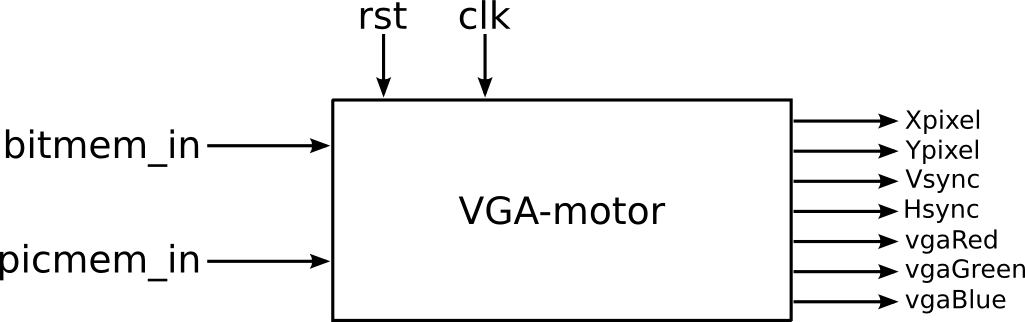
\includegraphics[width=1\textwidth]{drawings/vga_motor.png}}
	\caption{Översiktligt blockschema över VGA-motorn}
\end{figure}

VGA-motorn är ansvarig för att ta informationen från bildminnet och översätta detta till giltig VGA-output i form av RGB-signaler och H/V-sync för 640x480 pixlar i 60Hz. Den använder en klockfrekvens på 25Mhz. Denna används för att räkna upp \texttt{Xpixel} och \texttt{Ypixel}. Pixelräknarna används sedan för att generera \texttt{Vsync}, \texttt{Hsync} och \texttt{Blank}.

För varje pixel måste också ett utvärde beräknas. På vänster hälft (\texttt{Xpixel} < 320) av skärmen innehåller \texttt{bitmem\_in} information om ifall pixeln är svart (nolla) eller vit (etta). På höger hälft (\texttt{Xpixel} > 320) innehåller \texttt{picmem\_in} information om vilken tile som ska ritas upp. Se \ref{parag:picmempixel} för hur dessa uppdateras.

VGA-motorn har ett tileminne, \texttt{tileMem}, som innehåller 48 tecken (A-Ö, 0-9, samt ett par specialtecken) på 8x16 bitar vardera. Med hjälp av \texttt{picmem\_in} som väljer ut en tile, de sista fyra bitarna av \texttt{Xpixel} och de sista tre bitarna av \texttt{Ypixel} pekas en pixel i tileminnet ut. I \texttt{tileMem} är en svart pixel en etta och en vit pixel en nolla. 

En svart pixel fyller alla bitar i \texttt{vgaRed}, \texttt{vgaGreen} och \texttt{vgaBlue} med nollor, medans en vit pixel fyller dem med ettor. Om man ska läsa från \texttt{tileMem} eller \texttt{bitmem\_in} bestäms även här av \texttt{Xpixel}. En blanksignal ger samma resultat som en svart pixel.

\begin{figure}[h!]
	\makebox[\textwidth][c]{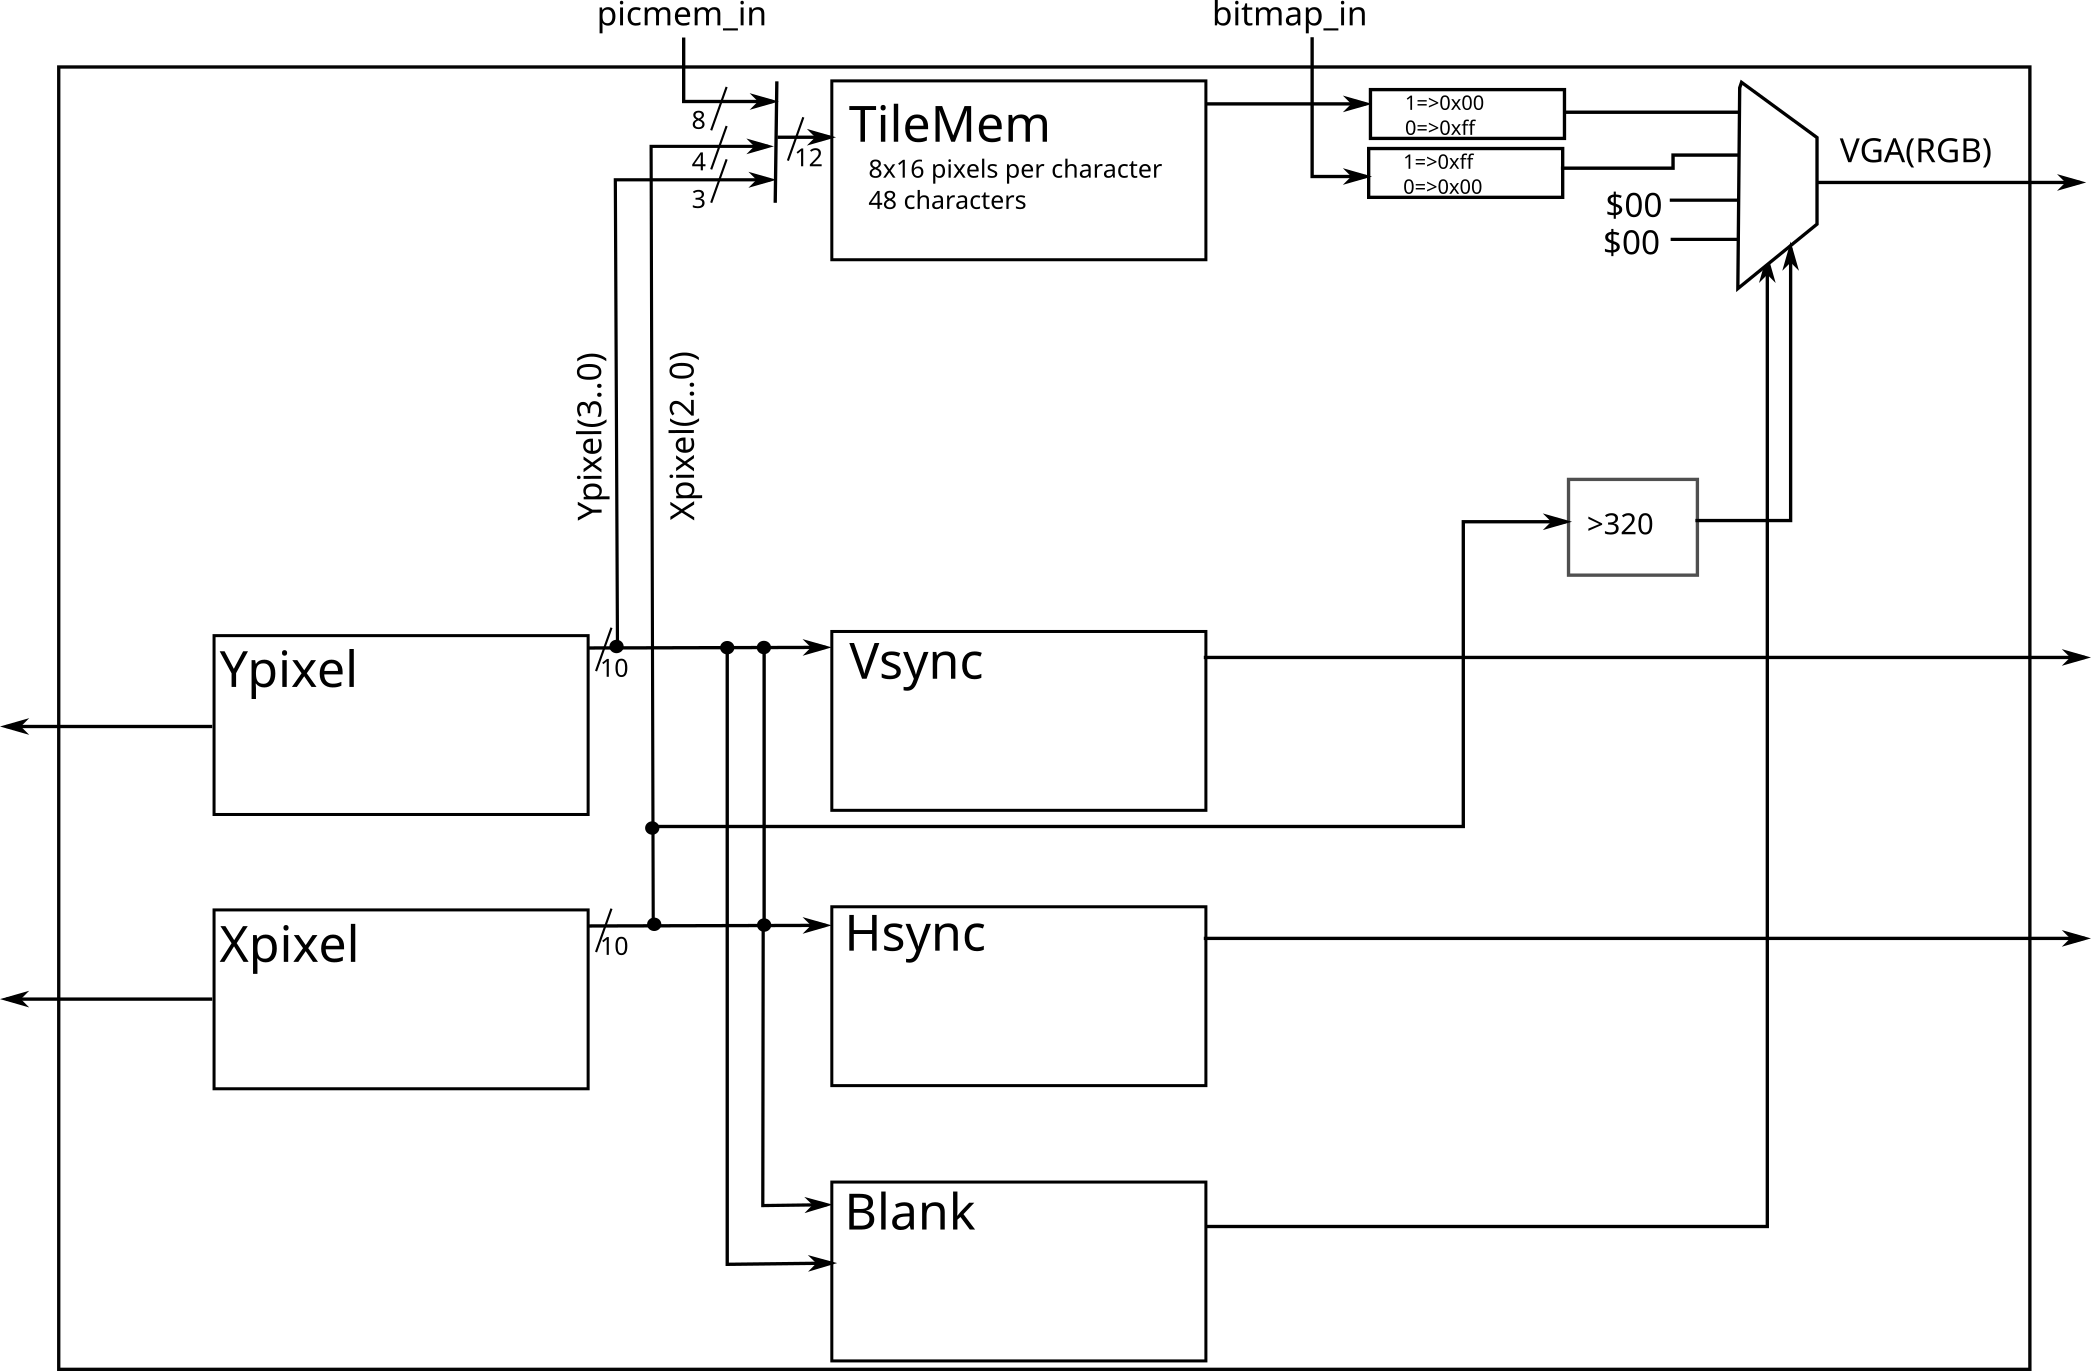
\includegraphics[width=1.3\textwidth]{drawings/vga_motor_detail.png}}
	\caption{Detaljerat blockschema över VGA-motorn}
\end{figure}

\newpage
\section{Mjukvara}

Använd de här tabellerna för ''subrutiner''\\


\begin{tabular}{ll}
	\textbf{GRx}    & \textbf{Input}        \\ \hline
	\texttt{0}      &  \\
	\texttt{1}      &  \\
	\texttt{2}      &  \\
	\texttt{Others} & Används ej till input \\
	                &  \\
	\textbf{GRx}    & \textbf{Output}       \\ \hline
	\texttt{0}      & Resultat
\end{tabular}


\subsection{Hjälpmedel}

\subsubsection{Sillescript}

Är ett relativt avancerat korsassembler-språk, vars kompilator är skriven i Python. I detta den stora majoriteten av koden är skriven.

Förutom att innehålla översättningar av alla instruktionsnamn till deras respektive binärkod finns även labels, kommentarer, if-satser (med support för else), while-satser, include-statements, och lite annat syntaktiskt socker.

Nedan följer ett utdrag ur koden som används för att byta ut ''X'' i ett funktionsuttryck mot ett visst värde.

\begin{oframed}
\begin{verbatim}
# Modify function: Replace X'es
load$ 0,0 # Loop counter
while 0 < &inputLength # GR0 < number of input elements
      
      # Put the value &nextInputType is 
      #   pointing to on GR2.
      load~ 2,&nextInputType

      if 2=$2 # If value is X
      	 # Replace the X in the function with proper Xval
      	 store~ 1,&nextInput
      end if

      ...

      # Increment loop counter
      add$ 0,1

      ...

end while

# Labels this row as inputLength. Start value: 8.
inputLength: sli 8
\end{verbatim}
\end{oframed}

\noindent
Syntax som bär uppmärksammas:\\

\begin{tabular}{p{2.5cm} p{8.5cm}}
\textbf{Syntax} & \textbf{Beskrivning}\\
\hline
\texttt{\#} & Kommentar.\\
: & Labeldefinition. ''Döper'' raden det är skrivet på till labelnamnet som ges innan kolonet.\\
Jämförelser & Vänsterledet avser alltid ett GRx. Siffran indikerar vilken av de 8. Högerledet är mer flexibelt, och kan ändras genom att använda tecknen nedan. Finns support för \texttt{=},\texttt{!},\texttt{>} och \texttt{<}.\\
\$ & Indikator. Säger att instruktionen skall körs med omedelbart mod. Om tecknet används i en jämförelse så indikerar det att följande värde är en literal.\\
\~{ }  & Indikator. Säger att instruktionen skall körs med indirekt mod.\\
\& & Indikator. Säger att det som följer är ett labelnamn. Detta namn översätts under kompilering till en korrekt address.\\
Ingen indikator & Säger att instruktionen skall körs med direkt mod. Om högerledet i en jämförelse saknar sådant tecken så indikerar det att värdet är en adress, och värdet sparat på adressen ska användas i jämförelsen.\\
\end{tabular}

\noindent
Nedan följer en lista på instruktioner som språket stödjer. Alla tar en mod (given via indikator), ett GRx (även om det inte används), och en address, literal, eller label.

\begin{multicols}{3}
\begin{itemize*}
\item load
\item store
\item add
\item addf
\item sub
\item subf
\item and
\item asl
\item asr
\item jmp
\item lsr
\item lsl
\item storep
\item rc
\item storeb
\item sli
\item include
\end{itemize*}
\end{multicols}

\noindent
Sli (''\textbf{s}et \textbf{li}ne'') och include är speciella, och har inte samma syntax som resten av instruktionerna; båda tar endast ett argument, och har varken support för moder, labels, eller indikatorer. Detta då de körs i kompileringstid, snarare än som maskinkod.

Sli följs av ett värde, och sätter raden som instruktionen befinner sig på till binärrepresentationen av det värdet.

Include följs av ett filnamn, och kopierar innehållet av den filen till filen som kompileras. En fil kan som mest inkluderas en gång. Flera inklusioner ger varningar och ignoreras.

För att faktiskt kompilera en Sillescript-fil så kan följande konsolkommando användas (då man sitter i projektets \texttt{sillescript2}-mapp):\\

\begin{Verbatim}[frame=single]
python compiler.py filename
\end{Verbatim}

\noindent
Detta skriver ut kompilerad output i konsolen, som sedan är ämnat att kopieras in i \texttt{cpu.vhd}-filen, på rätt plats. 

Pythonscriptet \texttt{compileAndLoad.py} kan dock göra detta åt dig; den kompilerar en fil och skriver sedan in resultatet i \texttt{cpu.vhd}. 

Notera att detta är i allra högsta grad specialanpassad för detta projekt, så omstrukturering av mappar, eller större ändringar i \texttt{cpu.vhd} kan få scriptet att sluta funka. Körs via:\\

\begin{Verbatim}[frame=single]
python compileAndLoad.py filename
\end{Verbatim}

\noindent
Scriptet sätter även en begränsning för när PM ska laddas med information från programminnet. Krävs för att det inte ska gå out of range när \texttt{ASR} sätts till något högre än storleken på \texttt{p\_mem}. Används inte \texttt{compileAndLoad.py} så bör denna begränsning sättas för hand.

\subsection{Testbänk}
Testbänken har förutom att generera en klocka på 100MHz även support för att skriva ut VGA-outputen tillsammans med tidsangivelser till en textfil. Denna kan sedan simuleras i en \href{http://ericeastwood.com/lab/vga-simulator/}{VGA-simulator}.


\subsection{''Subrutiner''}
\begin{figure}[h!]
	\makebox[\textwidth][c]{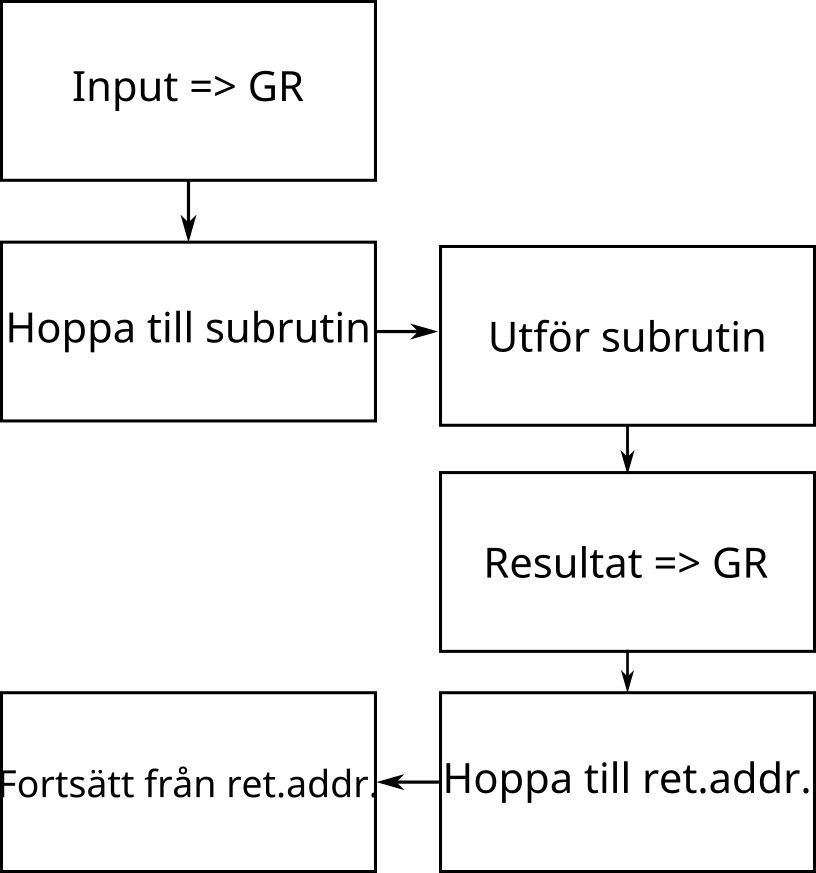
\includegraphics[width=0.4\textwidth]{drawings/subroutine.png}}
	\caption{Användandet av en ''subrutin''. }
\end{figure}

En subrutinsliknande struktur används för flera delar av programmet. Detta görs genom att ladda in input, däribland en returadress, till GR-register. Därefter hoppar den som vill kalla på ''subrutinen'' till ''subrutinens'' label. ''Subrutinen'' använder inputen för att utföra sin uppgift. Om returvärden behövs så sparar den det till ett eller flera förutbestämda GR. Sedan hoppar den till den specificerade returadressen. ''Subrutiner'' tar ingen hänsyn till att spara innehållet i register, utan det är anroparens uppgift att spara undan om det behövs. Dock används inga platser i dataminnet utanför dess egna block (TODO: Är detta sant?). Det finns i de flesta fall demoprogram för subrutiner vid namn \texttt{subrutinsnamn\_demo}.

\subsection{Omvandla inmatning till tal}\label{sec:text2hex}
För att omvandla en inmatad följd av siffror till ett enda tal i minnet använder vi koden i \texttt{text2hex}. Detta program väntar tills en giltig tangent registreras av tangentbordsmotorn (dvs. instruktionen \texttt{RC} läser in något annat värde än x$FF$) och avgör sedan om inmatningen är en operand (x$0$ - x$F$), operator ($+$, $-$, $*$, $/$, $=$), en särskild modifierare (\textit{P}, \textit{N}, \textit{R}) eller en särskild karaktär såsom \textit{X} eller mellanslag.

För att konstruera ett tal av en sifferföljd skiftas inmatningen ett lämpligt antal steg till vänster (16 steg för ett $4 \times 4$ fixpunktstal) så att inmatningen hamnar på de första fyra bitarna av heltalsdelen. Det tal som redan ligger i minnet skiftas sedan fyra steg till vänster och de två talen adderas. Se bilaga \ref{app:input_example} för ett exempel på denna process. Inmatning av decimaler fungerar på stort sett samma sett, men den nya siffran skiftas istället in till höger om punkten.

Den särskilda modifieraren \textit{N} (\textit{N}egative) kan användas för att ange att inmatningen ska tolkas som ett negativt tal, dvs inmatningsföljden ''\texttt{N5}'' betyder att värdet $-5$ ska sparas.

\subsection{Calc}
Koden i \texttt{calc} är huvudloopen i programmet, som inte hanterar enskilda inmatade siffror utan behandlar istället de hela tal, operatorer och modifierare som skickas vidare från \texttt{text2hex} (se sektion \ref{sec:text2hex}). Här avgörs det huruvida inmatningen ska läggas på evalueringsstacken (om tecknet är operand, operator, eller variabel \textit{X}), tolkas som en plotparameter (om inmatningen inleds med \textit{P}), eller är en särskild karaktär såsom \textit{R} (som rensar skärmen).

Detta bestäms i \texttt{calc} som sedan går vidare till lämplig 'subrutin' såsom \texttt{evaluate} eller \texttt{plot}. Dessa subrutiner återvänder sedan till \texttt{calc} som återställer relevanta variabler och register för nya inmatningar.

\subsection{Beräkningar}
\subsubsection{Reverse polish}
\begin{tabular}{ll}
	\textbf{GRx}    & \textbf{Input}               \\ \hline
	\texttt{0}      & Pekare till lista med värden \\
	\texttt{1}      & Pekare till lista med typer  \\
	\texttt{2}      & Storlek på listor            \\
	\texttt{3}      & Returadress                  \\
	\texttt{Others} & Används ej till input        \\
	                &  \\
	\textbf{GRx}    & \textbf{Output}              \\ \hline
	\texttt{0}      & Resultat av beräkning        \\
	\texttt{1}      & Beräkning lyckades
\end{tabular}
\\\\
\noindent
Listan som pekare GR0 pekar på innehåller alla värden för beräkningen i omvänd polsk notation. Operander kommer att sparas som sin adress i tileminnet, alltså 43=+, 44=-, 45=* och 46=/. För att särskilja operander från vanliga siffror används opvektorn som GR1 pekar på. Om det står 0 så är innehållet på samma index i värdesvektorn en siffra, om det står något annat så tolkas det som en operand. I övrigt följer evalueringen algoritmen från \href{https://en.wikipedia.org/wiki/Reverse_Polish_notation#Postfix_algorithm}{Wikipedia}. Stacken har en maxstorlek på 16 rader, därefter har den odefinierat resultat. 

När beräkningen är slutförd ligger resultatet i GR0 och en nolla i GR1. Ligger det någonting annat i GR1 så har beräkningen gått fel (felaktig input).

\subsubsection{Eval\_fn}

Byter ut ''X'' i ett uttryck mot nya värden, baserat på vilken pixel i X-led som nu ritas, och räknar sedan ut Y-värdet av funktionen vid den pixelkolumnen.

\begin{tabular}{ll}
	\textbf{GRx}    & \textbf{Input}               \\ \hline
	\texttt{0}      & Pekare till lista med värden \\
	\texttt{1}      & Pekare till lista med typer  \\
	\texttt{2}      & Storlek på listor            \\
	\texttt{3}      & Nuvarande X-pixel (heltal)   \\
	\texttt{4}      & Minsta X-värde på intervall (fixed-point) \\
	\texttt{5}      & Största X-värde på intervall (fixed-point) \\
        \texttt{6}      & Returadress                  \\
        \texttt{Others} & Används ej till input        \\
                        &                              \\
	\textbf{GRx}    & \textbf{Output}              \\ \hline
	\texttt{0}      & Resultat av beräkning: Y-värde (fixed-point) \\
	\texttt{1}      & 0 om lyckad beräkning, 1 annars
\end{tabular}
\\\\
\noindent
Värdelista tolkas på samma sätt som i \textit{Reverse polish}. Typlistan är också likadan, förutom skillnaden att en 2:a \textit{inte} tolkas som att en operator befinner sig på samma plats i värdelistan. Iställen tolkas en 2:a som att ett ''X'' finns på den platsen, och i värdelistan sätts då motsvarande X-värde in innan dessa automatiskt matas vidare till \textit{Reverse polish}. Samma stackbegränsningar gäller.

Minsta och största X-värden avser axelvärden efter skalning; om till exempel en graf ska ritas för X-värden mellan $-3.5$ och $8.47$, så anges dessa två värden. Därefter är det bara att ange motsvarande pixel. Rutinen antar att graffönstret är 320 pixlar brett, och given X-pixel förväntas därmed vara på intervallet 0 till 319.

När beräkningen är slutförd ligger resultatet i GR0 och en nolla i GR1. Ligger det någonting annat i GR1 så har beräkningen gått fel (felaktig input).

\subsubsection{Division}
\begin{tabular}{ll}
	\textbf{GRx}    & \textbf{Input}         \\ \hline
	\texttt{0}      & Täljare                \\
	\texttt{1}      & Nämnare                \\
	\texttt{2}      & Returadress            \\
	\texttt{Others} & Används ej till input  \\
	                &  \\
	\textbf{GRx}    & \textbf{Output}        \\ \hline
	\texttt{2}      & Resultat från division
\end{tabular}
\\\\
\noindent
Tar in ett en nämnare och en täljare och utför divisionen. Detta görs genom att subtrahera nämnaren från täljaren och räkna antalet subtraktioner. Försöker förbättra precisionen genom att skifta täljaren så långt till vänster som möjligt innan beräkningen, men kan ändå ge varierande bra resultat. Kommer ta mycket lång tid att utföra för vissa tal (små nämnare), upp till flera millisekunder. Efter beräkningen laddas resultatet till GR2 och programmet hoppar tillbaka till returadressen från inputen. En division med noll kommer ge noll som resultat.

\subsection{Grafer}

\subsubsection{DrawAxis}
\begin{tabular}{ll}
	\textbf{GRx}    & \textbf{Input}        \\ \hline
	\texttt{0}      & X-pixel               \\
	\texttt{1}      & Y-pixel               \\
	\texttt{2}      & Returadress           \\
	\texttt{Others} & Används ej till input \\
	             &  \\
	\textbf{GRx} & \textbf{Output}              \\ \hline
	             & Ingen output
\end{tabular}
\\\\
\noindent
Ritar grafaxlar med origo angivet som pixelkoordinater.

\subsubsection{Utritning: plot}
\begin{tabular}{ll}
	\textbf{GRx} & \textbf{Input}               \\ \hline
	\texttt{0}   & Minsta X-värde på intervall (fixed-point)  \\
	\texttt{1}   & Största X-värde på intervall (fixed-point) \\
	\texttt{2}   & Minsta Y-värde på intervall (fixed-point)  \\
	\texttt{3}   & Största Y-värde på intervall (fixed-point) \\
	\texttt{4}   & Pekare till lista med värden \\
	\texttt{5}   & Pekare till lista med typer  \\
	\texttt{6}   & Storlek på listor            \\
	\texttt{7}   & Returadress                  \\
	             &  \\
	\textbf{GRx} & \textbf{Output}              \\ \hline
	             & Ingen output
\end{tabular}
\\\\
\noindent
Argument följer samma logik som för \textit{Eval\_fn}.

Plot börjar med att beräkna skärmkoordinater för origo, och drawAxis tar sedan hand om den utritningen.

Därefter, för varje pixel i X-led så passeras argument till Eval\_fn, och motsvarande y-värde ritas ut. Detta skalas och översätts till ett pixelvärde baserat på given indata.

\subsection{IO}
\subsubsection{print\_num}
\begin{tabular}{ll}
	\textbf{GRx}    & \textbf{Input}                    \\ \hline
	\texttt{0}      & Nummer att skriva ut              \\
	\texttt{1}      & Adress i bildminnet att skriva på \\
	\texttt{2}      & Returadress                       \\
	\texttt{Others} & Används ej till input             \\
	                &  \\
	\textbf{GRx}    & \textbf{Output}                   \\ \hline
	                & Ingen output 						\\
\end{tabular}
\\\\
\noindent
Tar in ett fixed point-tal och skriver detta till specificerad adress med eventuellt minustecken framför. Skriver på formen ''0123.4567'' i hexadecimala tal. Tar alltså upp 9 tiles för positiva tal och 10 för negativa. Efter utskrivningen hoppar programmet tillbaka till returadressen från inputen.

\subsubsection{reset\_bitmap}
Skriver över alla pixlar i bitmapminnet med vitt. Är ingen subrutin, utan inkluderas där den ska användas.

\subsubsection{TODO}

\section{Slutsatser}
\section{Referenser}

\clearpage

\begin{appendices}
\section{Exempel på inmatning}\label{app:input_example}
Antag att användaren matar in sifferföljden "\textit{55}". Alltså förväntar sig användaren att talet x$53$ ska sparas i minne. Antag också att varje ny karaktär sparas till GR0, och det slutgiltiga talet ska sparas till GR1.

Vi observerar nu dessa register för att se hur x$53$ sparas.
\newline
\newline

Inledningsvis:
\begin{framed}
\begin{verbatim}
GR0: 0000 0000 0000 0000.0000 0000 0000 0000
GR1: 0000 0000 0000 0000.0000 0000 0000 0000
\end{verbatim}
\end{framed}

Inmatning: GR0 := 5
\begin{framed}
\begin{verbatim}
GR0: 0000 0000 0000 0000.0000 0000 0000 0101
GR1: 0000 0000 0000 0000.0000 0000 0000 0000
\end{verbatim}
\end{framed}

GR0 skiftas vänster 16 steg
\begin{framed}
\begin{verbatim}
GR0: 0000 0000 0000 0101.0000 0000 0000 0000
GR1: 0000 0000 0000 0000.0000 0000 0000 0000
\end{verbatim}
\end{framed}

GR1 skiftas vänster 4 steg
\begin{framed}
\begin{verbatim}
GR0: 0000 0000 0000 0101.0000 0000 0000 0000
GR1: 0000 0000 0000 0000.0000 0000 0000 0000
\end{verbatim}
\end{framed}

GR1 := GR1 + GR0
\begin{framed}
\begin{verbatim}
GR0: 0000 0000 0000 0101.0000 0000 0000 0000
GR1: 0000 0000 0000 0101.0000 0000 0000 0000
\end{verbatim}
\end{framed}

\newpage

Inmatning: GR0 := 3
\begin{framed}
\begin{verbatim}
GR0: 0000 0000 0000 0000.0000 0000 0000 0011
GR1: 0000 0000 0000 0101.0000 0000 0000 0000
\end{verbatim}
\end{framed}

GR0 skiftas vänster 16 steg
\begin{framed}
\begin{verbatim}
GR0: 0000 0000 0000 0011.0000 0000 0000 0000
GR1: 0000 0000 0000 0101.0000 0000 0000 0000
\end{verbatim}
\end{framed}

GR1 skiftas vänster 4 steg
\begin{framed}
\begin{verbatim}
GR0: 0000 0000 0000 0011.0000 0000 0000 0000
GR1: 0000 0000 0101 0000.0000 0000 0000 0000
\end{verbatim}
\end{framed}

GR1 := GR1 + GR0
\begin{framed}
\begin{verbatim}
GR0: 0000 0000 0000 0011.0000 0000 0000 0000
GR1: 0000 0000 0101 0011.0000 0000 0000 0000
\end{verbatim}
\end{framed}

GR1 innehåller nu bitrepresentatinen av x$53$ för ett $4 \times 4$ fixpunktstal.
\end{appendices}
\end{document}          
